\documentclass[11pt,a4paper]{article}
\usepackage[T1]{fontenc}
\usepackage[utf8]{inputenc}
\usepackage{lmodern,microtype}
\usepackage[margin=27mm,headheight=15pt]{geometry}
\usepackage{amsmath,amssymb,amsthm,mathtools}
\usepackage{xcolor,booktabs,array,longtable,enumitem,needspace}
\usepackage{tikz}
\usetikzlibrary{arrows.meta,positioning,fit,backgrounds}
\usepackage{fancyhdr}
\usepackage[colorlinks=true,linkcolor=blue!45!black,urlcolor=blue!45!black,citecolor=blue!45!black]{hyperref}
\usepackage[nameinlink,noabbrev]{cleveref}
\usepackage{listings}
\definecolor{ink}{HTML}{17364D}
\definecolor{soft}{HTML}{F2F5F7}
\hypersetup{pdftitle={Parikh's Theorem: A Constructive Proof for Formalization},pdfauthor={Prepared for Umang Mathur}}
\pagestyle{fancy}
\fancyhf{}\fancyhead[L]{\small\color{ink}Parikh's theorem}
\fancyhead[R]{\small A constructive proof}\fancyfoot[C]{\thepage}
\renewcommand{\headrulewidth}{0.3pt}
\setlength{\parindent}{0pt}\setlength{\parskip}{6pt plus 1pt minus 1pt}
\setlist{topsep=4pt,itemsep=3pt,parsep=0pt}
\setcounter{tocdepth}{2}
\newcolumntype{L}[1]{>{\raggedright\arraybackslash}p{#1}}
\numberwithin{equation}{section}
\theoremstyle{plain}
\newtheorem{theorem}{Theorem}[section]
\newtheorem{lemma}[theorem]{Lemma}
\newtheorem{proposition}[theorem]{Proposition}
\newtheorem{corollary}[theorem]{Corollary}
\theoremstyle{definition}
\newtheorem{definition}[theorem]{Definition}
\newtheorem{example}[theorem]{Example}
\theoremstyle{remark}
\newtheorem{remark}[theorem]{Remark}
\newcommand{\N}{\mathbb N}
\newcommand{\eps}{\varepsilon}
\newcommand{\wt}{\operatorname{wt}}
\newcommand{\supp}{\operatorname{supp}}
\newcommand{\rt}{\operatorname{root}}
\newcommand{\treeheight}{\operatorname{ht}}
\newcommand{\sz}{\operatorname{size}}
\newcommand{\yield}{\operatorname{yield}}
\newcommand{\front}{\operatorname{front}}
\newcommand{\Lin}{\operatorname{Lin}}
\newcommand{\Act}{\operatorname{Act}}
\newcommand{\Trees}{\mathcal T}
\newcommand{\Bases}{\mathcal B}
\newcommand{\Cycles}{\mathcal C}
\newcommand{\hole}[1]{\square_{#1}}
\newcommand{\llbracket}{\mathopen{[\![}}
\newcommand{\rrbracket}{\mathclose{]\!]}}
\newcommand{\ins}[1]{\xrightarrow{\;#1\;}}
\newcommand{\key}[1]{\begin{quote}\small\color{ink}\textbf{Key point.} #1\end{quote}}
\lstset{basicstyle=\small\ttfamily,columns=fullflexible,keepspaces=true,frame=single,rulecolor=\color{black!15},backgroundcolor=\color{soft},breaklines=true,showstringspaces=false}
\begin{document}
\begin{titlepage}
\vspace*{15mm}
{\small\sffamily\color{ink}FORMAL LANGUAGES\quad /\quad PROOF DEVELOPMENT}\par
\vspace{9mm}
{\Huge\bfseries Parikh's Theorem}\par
\vspace{4mm}
{\Large A constructive proof for formalization}\par
\vspace{12mm}
{\large A systematic and pedagogical exposition}\par
\vspace{6mm}
Prepared for Umang Mathur\par
11 October 2026
\vspace{13mm}
\hrule
\vspace{5mm}
\textbf{The result.} The Parikh image of every context-free language is a finite union of linear sets. Conversely, every semilinear set is the Parikh image of a regular language.

\textbf{The method.} Cut a derivation tree into a small complete tree and bounded one-hole contexts. Record which contexts occur at least once. Prove that, once these contexts have been introduced, their multiplicities can vary independently.

\textbf{The intended use.} This is a mathematical blueprint for mechanization. Definitions, induction measures, compatibility conditions, and both inclusions of the final set equality are explicit. The document contains no claimed machine-checked proof or dependency on a particular proof-assistant library.
\vspace{5mm}
\hrule
\vfill
\small
The proof works with arbitrary finite context-free grammars. Empty right-hand sides, unit productions, unproductive symbols, and ambiguous derivations require no preprocessing. All natural numbers include zero.
\end{titlepage}

{\small\setlength{\parskip}{0pt}\tableofcontents}
\newpage

\section{The statement and the proof contract}\label{sec:statement}

\subsection{Words become vectors}
Fix a finite terminal alphabet $\Sigma$. We use $\N^\Sigma$ for the set of functions from $\Sigma$ to $\N$, with pointwise addition. This avoids choosing an order on the alphabet. If $\Sigma=\{a_1,\ldots,a_d\}$ has been ordered, this is simply $\N^d$.

\begin{definition}[Parikh map]
For a word $w\in\Sigma^*$, its Parikh vector $\Psi(w)\in\N^\Sigma$ is defined by
\[
\Psi(w)(a)=\text{the number of occurrences of $a$ in $w$}.
\]
For a language $L\subseteq\Sigma^*$, let $\Psi(L)=\{\Psi(w):w\in L\}$.
\end{definition}

For example, over the ordered alphabet $(a,b,c)$,
\[
\Psi(\texttt{abacb})=(2,2,1)=\Psi(\texttt{bbaac}).
\]
The two words differ, but their counts agree. Write $e_a$ for the vector with value $1$ at $a$ and $0$ elsewhere. Directly from counting,
\begin{equation}\label{eq:word-add}
\Psi(\eps)=0,\qquad \Psi(a)=e_a,\qquad
\Psi(uv)=\Psi(u)+\Psi(v).
\end{equation}
For the last identity, fix a letter $a$. Its occurrences in $uv$ split into the occurrences in $u$ and those in $v$. Equality at every coordinate gives equality of vectors. Induction then gives additivity for any finite concatenation and $\Psi(w^k)=k\Psi(w)$.

\subsection{Linear and semilinear sets}
\begin{definition}[Linear set]
For a base vector $b\in\N^\Sigma$ and a finite indexed family of period vectors $(p_i)_{i\in I}$, define
\[
\Lin(b;(p_i)_{i\in I})
=\left\{b+\sum_{i\in I}k_i p_i : (k_i)_{i\in I}\in\N^I\right\}.
\]
A set is \emph{linear} if it has this form, and \emph{semilinear} if it is a finite union of linear sets.
\end{definition}

The empty index set gives $\Lin(b;())=\{b\}$. The empty union gives $\varnothing$. A period may be zero, and different indices may carry the same period vector. These conventions are useful for grammars with silent cycles.

\begin{example}
The set $\{(n,n):n\in\N\}$ is linear, with base $(0,0)$ and period $(1,1)$. The set
\[
\{(2+3m,n):m,n\in\N\}\ \cup\ \{(0,0)\}
\]
is semilinear: its first component has base $(2,0)$ and periods $(3,0),(0,1)$; its second component is a singleton.
\end{example}

\begin{theorem}[Parikh's theorem, with its converse]\label{thm:parikh-statement}
For every finite context-free grammar $G$ over $\Sigma$, the set $\Psi(L(G))$ is semilinear. Moreover, the proof gives an effective procedure to obtain a finite semilinear representation from $G$, with explicit grammar-dependent bounds on the number of components, the number of periods, and all vector magnitudes (\cref{thm:size-bound}).

Conversely, for every semilinear set $X\subseteq\N^\Sigma$, one can effectively construct a regular language $R\subseteq\Sigma^*$ such that $\Psi(R)=X$.
\end{theorem}

Thus every context-free language has the same Parikh image as some regular language. This statement does \emph{not} say that the original language is regular, or that every language with that Parikh image is context-free.

For instance, $\{a^n b^n c^n:n\in\N\}$ and $(abc)^*$ have the same Parikh image, although the former is not context-free. This familiar example is only an illustration; its non-context-freeness is not used in the proof.

\subsection{What the proof will establish}
We will define a finite set $\Bases$ of complete trees and a finite set $\Cycles$ of repeatable contexts. For each $B\in\Bases$ and each suitable subset $D\subseteq\Cycles$, the proof constructs a linear set
\begin{equation}\label{eq:preview}
\left\{\wt(B)+\sum_{C\in D}\wt(C)
       +\sum_{C\in D}k_C\wt(C):k_C\in\N\right\}.
\end{equation}
The first sum pays for \emph{one occurrence of every chosen context}. The second sum accounts for additional occurrences. We will prove that the union of precisely these components is $\Psi(L(G))$.

The word ``suitable'' matters. A context rooted at $A$ can only be inserted into a tree that contains an $A$-node. One context may introduce the nonterminal needed by another. Establishing this compatibility condition is the central combinatorial issue after tree decomposition.

\section{A map of the argument}\label{sec:map}

\textbf{A first picture.} For the grammar $S\to aSb\mid\eps$, start with the tree using $S\to\eps$. Surround its $S$-root with the context for $S\to a\hole S b$. Each such insertion adds one $a$ and one $b$. After $r$ insertions the yield is $a^r b^r$ and the count vector is $r(1,1)$. A small tree plus repeatable additions has produced a linear set. For a general grammar there are several kinds of additions, and we must also determine which kinds can coexist.

The argument has five stages. Each stage isolates a different proof obligation.
\begin{enumerate}
\item \textbf{Local surgery.} A context with an $A$-root and one $A$-hole can surround an existing $A$-subtree. The result is still a valid derivation tree. Terminal counts add, and the set of nonterminals present can only grow.
\item \textbf{Bounded decomposition.} Repeatedly remove a bounded context from a non-simple tree. The number of production nodes strictly decreases, so the process terminates at a simple complete tree.
\item \textbf{Activation.} From a valid insertion sequence, retain contexts in order of first occurrence. Each retained context is still enabled. After this first pass, all retained contexts can be inserted arbitrarily often.
\item \textbf{Finite union.} There are finitely many simple complete trees, finitely many bounded contexts, and finitely many subsets of those contexts. Each compatible pair gives exactly one linear component.
\item \textbf{Converse.} Realize a base vector by one word and each period vector by another word. A finite union of expressions of the form $u v_1^*\cdots v_k^*$ has the required Parikh image.
\end{enumerate}

\begin{center}
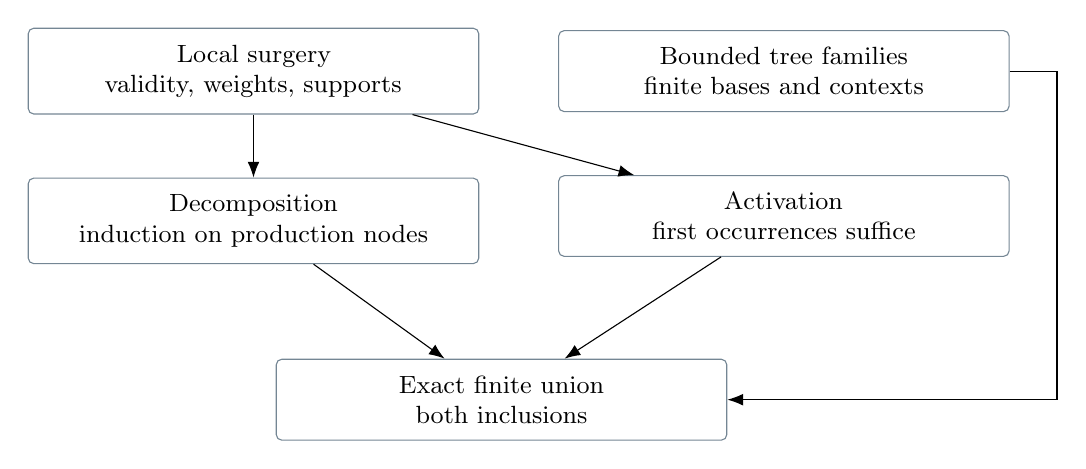
\begin{tikzpicture}[node distance=8mm and 10mm,
 box/.style={draw=ink!60,rounded corners=2pt,align=center,text width=53mm,inner sep=6pt,font=\small},
 >={Latex[length=2mm]}]
\node[box] (surgery) {Local surgery\\validity, weights, supports};
\node[box,right=of surgery] (finite) {Bounded tree families\\finite bases and contexts};
\node[box,below=of surgery] (decomp) {Decomposition\\induction on production nodes};
\node[box,below=of finite] (activation) {Activation\\first occurrences suffice};
\node[box,below=12mm of decomp,xshift=31.5mm] (main) {Exact finite union\\both inclusions};
\draw[->] (surgery)--(decomp);
\draw[->] (surgery)--(activation);
\draw[->] (finite.east) -- ++(6mm,0) |- (main.east);
\draw[->] (decomp)--(main);
\draw[->] (activation)--(main);
\end{tikzpicture}
\end{center}

\textbf{Reading order.} Sections~\ref{sec:trees}--\ref{sec:main} contain the complete forward proof. Section~\ref{sec:example} is a worked example of the subtle activation step. Section~\ref{sec:converse} proves the converse. Sections~\ref{sec:effective} and~\ref{sec:formalization} explain effective construction and mechanization. The appendices supply the connection to ordinary word derivations and a small arithmetic corollary.

\textbf{Dependencies.} The forward proof uses induction on finite trees and natural numbers, finite enumeration, and elementary arithmetic in $\N^\Sigma$. It does not invoke a grammar normal form, the pumping lemma, Dickson's lemma, a theorem about Diophantine equations, or Presburger quantifier elimination.

\section{Grammars and derivation trees}\label{sec:trees}

\subsection{The grammar model}
Fix a grammar $G=(N,\Sigma,P,S)$, where $N$ and $\Sigma$ are disjoint finite sets, $S\in N$, and $P$ is a finite set of productions
\[
A\to X_1\cdots X_m,
\qquad A\in N,\quad X_i\in N\uplus\Sigma,\quad m\geq 0.
\]
The disjoint union notation records whether a symbol is a nonterminal or a terminal. Let $n=|N|$. Since $S\in N$, we have $n\geq1$.

A sentential form is a word over $N\uplus\Sigma$. The relation $\alpha\Rightarrow_G\beta$ means that one occurrence of some $A$ in $\alpha$ is replaced by the right-hand side of a production for $A$. Its reflexive transitive closure is $\Rightarrow_G^*$. The generated language is
\[
L(G)=\{w\in\Sigma^*:S\Rightarrow_G^*w\}.
\]
There are no restrictions on right-hand sides. In particular, $A\to\eps$ and $A\to B$ are permitted.

\subsection{A representation that handles empty productions correctly}
\begin{definition}[Complete grammar tree]\label{def:tree}
A complete grammar tree is built using the following constructors.
\begin{itemize}
\item For each $a\in\Sigma$, $\operatorname{leaf}(a)$ is a tree with root symbol $a$.
\item If $p=(A\to X_1\cdots X_m)\in P$ and $T_1,\ldots,T_m$ are complete trees with root symbols $X_1,\ldots,X_m$, then
\[
\operatorname{node}(p;T_1,\ldots,T_m)
\]
is a complete tree with root symbol $A$.
\end{itemize}
Write $\Trees_A$ for the complete trees with root symbol $A\in N$.
\end{definition}

Children are ordered. A production node carries its production, not merely its left-hand nonterminal. This records the local validity evidence explicitly. A node for $A\to\eps$ has no children and is a \emph{production node}, even though it is a leaf of the underlying graph. It is not an unexpanded $A$.

\begin{definition}[Yield, weight, size, height, and support]\label{def:statistics}
For complete trees, define
\begin{align*}
\yield(\operatorname{leaf}(a))&=a,&
\yield(\operatorname{node}(p;T_1,\ldots,T_m))&=\yield(T_1)\cdots\yield(T_m),\\
\wt(T)&=\Psi(\yield(T)),\\
\sz(\operatorname{leaf}(a))&=0,&
\sz(\operatorname{node}(p;T_1,\ldots,T_m))&=1+\sum_{i=1}^m\sz(T_i),\\
\treeheight(\operatorname{leaf}(a))&=0,&
\treeheight(\operatorname{node}(p;T_1,\ldots,T_m))&=1+\max_i\treeheight(T_i),\\
\supp(\operatorname{leaf}(a))&=\varnothing,&
\supp(\operatorname{node}(p;T_1,\ldots,T_m))&=\{A\}\cup\bigcup_i\supp(T_i),
\end{align*}
where $A$ is the left-hand side of $p$ and the maximum of an empty family is $0$.
\end{definition}

Thus size counts production nodes, height counts production nodes along a longest path, and support records which nonterminals label production nodes. For $p=(A\to\eps)$, the tree $\operatorname{node}(p;)$ has yield $\eps$, weight $0$, size $1$, height $1$, and support $\{A\}$.

\begin{proposition}[Trees and word derivations]\label{prop:tree-word}
For every $A\in N$ and $w\in\Sigma^*$,
\[
A\Rightarrow_G^*w
\quad\Longleftrightarrow\quad
\exists T\in\Trees_A\;\;\yield(T)=w.
\]
Consequently $\Psi(L(G))=\{\wt(T):T\in\Trees_S\}$.
\end{proposition}
\begin{proof}
A complete proof, using partial trees to track a word derivation one step at a time, is given in Appendix~\ref{app:derivations}. The forward proof below uses only the displayed consequence.
\end{proof}

\subsection{Occurrences are positions, not just labels}
A position in an ordered tree is a finite sequence of child indices. The empty sequence $\eps$ names the root. If $q$ names a node with $m$ children, then $qi$ names its $i$th child, for $1\leq i\leq m$. Write $T|_q$ for the subtree at $q$.

If $q$ names a production node, replacing $T|_q$ by any complete tree with the same root symbol preserves local validity: the parent still sees the same child-root symbol, and all other productions are unchanged. At the root there is no parent, and the root symbol is preserved directly.

\key{An insertion is made at a particular occurrence of a nonterminal. The support set tells us that a suitable occurrence exists; the position tells us where to perform the insertion.}

\section{Contexts and the local surgery lemmas}\label{sec:contexts}

\subsection{One distinguished hole}
Extend the tree syntax with a constructor $\hole{A}$ for each $A\in N$. Its root symbol is $A$. It is not a production node. In a production node, a hole may occupy a child position whose required root symbol is its label, and holes may also occur deeper in its children.

An \emph{open grammar tree} is a tree in this extended syntax satisfying the same production and child-root conditions. A \emph{one-hole context} is an open grammar tree containing exactly one hole. Complete trees contain no holes. If $E$ has hole $\hole{A}$ and $T\in\Trees_A$, let $E[T]$ be the tree obtained by replacing that hole by $T$.

For an open tree, define weight by summing $e_a$ over all terminal leaves. Define size, height, and support by the same recursions as before, with
\[
\wt(\hole{A})=0,\qquad\sz(\hole{A})=0,\qquad
\treeheight(\hole{A})=0,\qquad\supp(\hole{A})=\varnothing.
\]
In particular, \emph{the hole does not contribute its label to support}. This convention makes support under plugging exactly additive by union.

\begin{definition}[Cycle context]\label{def:cycle}
A cycle context is a valid one-hole context $C$ whose root symbol and hole label are the same nonterminal $A$, and which is not the one-node context $\hole{A}$. Write $\rt(C)=A$.
\end{definition}

The word ``cycle'' refers to returning from $A$ to another occurrence of $A$ along the path to the hole. The tree itself is finite and acyclic. A cycle context contains at least one production node, so
\begin{equation}\label{eq:cycle-root}
\sz(C)\geq1,\qquad \rt(C)\in\supp(C).
\end{equation}
Its terminal frontier has the form $u\hole{A}v$, for terminal words $u,v$. Consequently $\wt(C)=\Psi(u)+\Psi(v)$. The hole is a placeholder; its label is not counted as a terminal.

\begin{lemma}[Plugging identities]\label{lem:plug}
Let $E$ be a valid one-hole context with hole $\hole{A}$, and let $T\in\Trees_A$. Then $E[T]$ is complete and valid, has the root symbol of $E$, and satisfies
\begin{align}
\wt(E[T])&=\wt(E)+\wt(T),\label{eq:plug-wt}\\
\sz(E[T])&=\sz(E)+\sz(T),\label{eq:plug-size}\\
\supp(E[T])&=\supp(E)\cup\supp(T).\label{eq:plug-supp}
\end{align}
\end{lemma}
\begin{proof}
Induct on the number of edges from the root of $E$ to its unique hole.

If that number is zero, then $E=\hole{A}$ and $E[T]=T$. All claims follow from the definitions for a hole.

Otherwise the root is a production node. Exactly one child, say the $j$th, contains the hole. The other children are complete. Apply the induction hypothesis to the $j$th child and leave all other children unchanged. The replaced child retains its root symbol, so the production at the root remains valid. There is no hole after replacement.

At a production node, weight is the sum of child weights, size is one plus the sum of child sizes, and support is the union of the root label and child supports. Substituting the three induction identities into these recursions proves all three displayed equations. The root production is unchanged, hence so is its root symbol.
\end{proof}

\subsection{Inserting a cycle into a complete tree}
\begin{definition}[Insertion]\label{def:insertion}
For complete nonterminal-rooted trees $T,T'$ and a cycle context $C$ with root $A$, write $T\ins C T'$ if there is a production-node position $q$ of $T$ with root label $A$ such that $T'$ is obtained by replacing $T|_q$ with $C[T|_q]$.
\end{definition}

The old subtree is retained inside the new context. We insert structure around it; we do not discard it.

\begin{lemma}[Insertion is enabled exactly by support]\label{lem:enabled}
For a complete nonterminal-rooted tree $T$ and a cycle context $C$, there exists $T'$ with $T\ins C T'$ if and only if $\rt(C)\in\supp(T)$.
\end{lemma}
\begin{proof}
An insertion supplies a production-node occurrence of $\rt(C)$, so the label lies in support. Conversely, membership in support supplies such a position $q$. Plug $T|_q$ into $C$ and replace the subtree at $q$. The plugging lemma and equality of root labels give a valid complete tree.
\end{proof}

\begin{lemma}[Insertion preserves the old tree's resources]\label{lem:insertion-laws}
If $T\ins C T'$, then $T'$ has the same root symbol as $T$, and
\begin{align}
\wt(T')&=\wt(T)+\wt(C),\label{eq:insert-wt}\\
\sz(T')&=\sz(T)+\sz(C),\label{eq:insert-size}\\
\supp(T')&=\supp(T)\cup\supp(C).\label{eq:insert-supp}
\end{align}
\end{lemma}
\begin{proof}
Let $U=T|_q$ be the selected subtree and let $E$ be the outer context obtained from $T$ by replacing $U$ by a hole of the same root label. Then
\[
T=E[U],\qquad T'=E[C[U]].
\]
Apply \cref{lem:plug} first to $C[U]$ and then to the outer plugging by $E$. For weight and size, associate and commute addition. For support, associate and commute union. The outer context gives the same root symbol in both trees.
\end{proof}

\begin{corollary}[Accounting along an insertion sequence]\label{cor:sequence}
If
\[
T_0\ins{C_1}T_1\ins{C_2}\cdots\ins{C_m}T_m,
\]
then
\begin{align*}
\wt(T_m)&=\wt(T_0)+\sum_{i=1}^m\wt(C_i),\\
\supp(T_m)&=\supp(T_0)\cup\bigcup_{i=1}^m\supp(C_i).
\end{align*}
Every intermediate tree is complete and has the root symbol of $T_0$.
\end{corollary}
\begin{proof}
Induct on $m$ and apply \cref{lem:insertion-laws} at the last step. For $m=0$, the sum and union over contexts are empty.
\end{proof}

\key{Future insertions depend only on the presence of nonterminal labels. Insertion never removes a label that was already present. This monotonicity will let us discard repeated uses while deciding which contexts can be activated.}

\section{Finite building blocks and exact decomposition}\label{sec:decomposition}

\subsection{Simple trees}
\begin{definition}[Simple complete tree]
A complete tree is simple if no root-to-leaf path contains two production nodes with the same nonterminal label.
\end{definition}

Repeated labels in different branches are permitted. For example, a tree for $S\to AA$, with each $A\to a$, is simple when $S\neq A$. Simplicity is a condition on each path, not on the total number of occurrences of a label in the whole tree.

\begin{lemma}[Height of a simple tree]\label{lem:simple-height}
Every simple complete tree has height at most $n=|N|$.
\end{lemma}
\begin{proof}
Along any path, the production-node labels are pairwise distinct members of the $n$-element set $N$. The path therefore contains at most $n$ production nodes. Taking the maximum over paths gives the height bound. A terminal-only tree has height zero and also satisfies it.
\end{proof}

\begin{definition}[The two finite families]\label{def:families}
Let
\begin{align*}
\Bases&=\{B\in\Trees_S:B\text{ is simple}\},\\
\Cycles&=\{C:C\text{ is a cycle context and }\treeheight(C)\leq n+1\}.
\end{align*}
\end{definition}

We deliberately put \emph{all} bounded valid cycle contexts in $\Cycles$. We do not require that a context has already appeared in some successful derivation from $S$. Such a requirement would complicate effective enumeration. The activation condition will reject contexts that cannot be used with a particular base.

\begin{lemma}[Finiteness and effective enumeration]\label{lem:finite}
For every $H\in\N$, there are finitely many valid open grammar trees of height at most $H$, and they can be effectively enumerated. Consequently $\Bases$ and $\Cycles$ are finite and effectively enumerable.
\end{lemma}
\begin{proof}
At height zero, the only possibilities are terminal leaves and holes. There are finitely many of both because $\Sigma$ and $N$ are finite.

Suppose the family at height at most $H$ is finite and enumerable. A tree of height at most $H+1$ is either a terminal leaf, a hole, or a production node $\operatorname{node}(p;T_1,\ldots,T_m)$. There are finitely many choices for $p\in P$. For a fixed $p$, its arity $m$ is fixed and finite. Each child comes from the enumerated family at height at most $H$. Enumerate the finite Cartesian product of these child families, and retain tuples whose root symbols match the right-hand side of $p$. This generates precisely the valid trees at the new bound.

For $\Bases$, enumerate to height $n$ and filter for no holes, root $S$, and simplicity. The height lemma shows that every simple $S$-tree is included. For $\Cycles$, enumerate to height $n+1$ and filter for exactly one hole, matching root and hole labels, and nontriviality. All these tests concern finite trees and are decidable.
\end{proof}

\subsection{The bounded cut}
An arbitrary repetition in a large tree may enclose very large side branches. Cutting there would not immediately give a bounded context. We instead locate a non-simple subtree whose proper subtrees are all simple.

\begin{lemma}[A non-simple tree contains a bounded removable context]\label{lem:cut}
Let $T\in\Trees_A$ be non-simple. Then there exist $T'\in\Trees_A$ and $C\in\Cycles$ such that
\[
T'\ins C T\qquad\text{and}\qquad\sz(T')<\sz(T).
\]
The insertion reconstructs $T$ exactly, including its production labels and child order.
\end{lemma}
\begin{proof}
\textbf{1. Choose a minimal non-simple subtree.}
Among the non-simple subtrees of $T$, choose one, $U$, with the least number of production nodes. This is a nonempty finite collection because $T$ itself is non-simple. Every proper nonterminal-rooted subtree of $U$ is smaller than $U$ and hence simple. Terminal-rooted subtrees are simple as well.

\textbf{2. The repeated label must include the root.}
Let the root label of $U$ be $B$. Because $U$ is non-simple, some path has a repeated nonterminal. If both occurrences were strictly below the root, they would lie in one child subtree of $U$, contradicting simplicity of that subtree. Thus $B$ occurs again at a proper descendant production node. Choose one such occurrence, and let $V$ be its complete $B$-rooted subtree.

\textbf{3. Extract the context.}
Replace this occurrence of $V$ in $U$ by $\hole{B}$; call the resulting open tree $C$. It has exactly one hole. Its root and hole label are both $B$. Since the chosen occurrence was a proper descendant, the original root production remains, so $C$ is nontrivial. All unchanged productions remain valid, and the replacement hole has the required root symbol. Therefore $C$ is a cycle context and $U=C[V]$.

\textbf{4. Bound its height.}
Each child subtree of $U$ is simple and therefore has height at most $n$. Hence $\treeheight(U)\leq n+1$. Replacing a subtree by a height-zero hole cannot increase height, so $\treeheight(C)\leq n+1$. Thus $C\in\Cycles$.

\textbf{5. Cut it out of the original tree.}
Let $E$ be the outer context selecting the occurrence of $U$ in $T$. Then
\[
T=E[U]=E[C[V]].
\]
Define $T'=E[V]$. Since $U$ and $V$ have the same root label, $T'$ is a complete valid $A$-tree. Inserting $C$ at the occurrence of $V$ gives $T$ exactly. The size identities give
\[
\sz(T)=\sz(E)+\sz(C)+\sz(V)
         =\sz(T')+\sz(C)>\sz(T'),
\]
because $\sz(C)\geq1$.
\end{proof}

\key{The decrease is in production-node count, not terminal yield length. A removable context may produce no terminal letters at all.}

\subsection{Decomposing every complete tree}
\begin{theorem}[Exact decomposition]\label{thm:decomposition}
For every complete $A$-rooted tree $T$, there exist a simple complete $A$-rooted tree $B$ and a finite insertion sequence
\begin{equation}\label{eq:decomposition}
B=T_0\ins{C_1}T_1\ins{C_2}\cdots\ins{C_m}T_m=T
\end{equation}
with $C_i\in\Cycles$ for every $i$. If $A=S$, then $B\in\Bases$.
\end{theorem}
\begin{proof}
Use strong induction on $\sz(T)$, with the statement quantified over all root nonterminals and all trees of that size.

If $T$ is simple, take $B=T$ and the empty sequence. Otherwise, \cref{lem:cut} gives $T'$ and $C\in\Cycles$ with $\sz(T')<\sz(T)$ and $T'\ins C T$. Apply the induction hypothesis to $T'$. It supplies a simple tree $B$ of the same root and a sequence from $B$ to $T'$ using contexts in $\Cycles$. Append the single insertion $T'\ins C T$. The resulting sequence has all required properties.
\end{proof}

There is no uniqueness claim. Different minimal subtrees or repeated occurrences can lead to different decompositions. Existence is enough. If a deterministic algorithm is wanted, fix orders on productions and child positions and always take the first eligible choice.

\begin{corollary}[Exact generation by the finite families]\label{cor:finite-generation}
The complete $S$-rooted trees are exactly the trees obtainable from some $B\in\Bases$ by a finite valid sequence of insertions of contexts from $\Cycles$.
\end{corollary}
\begin{proof}
The forward inclusion is \cref{thm:decomposition}. For the reverse inclusion, a base is a complete $S$-tree and every insertion preserves completeness, grammar validity, and root symbol by \cref{lem:insertion-laws}.
\end{proof}

\section{Which sets of contexts can be used together?}\label{sec:activation}

Fix a complete nonterminal-rooted tree $B$ and a finite set $D$ of cycle contexts. For this section, $B$ need not be simple and the contexts need not have bounded height. This separates the activation argument from the particular bounds of the preceding section.

\subsection{An explicit compatibility condition}
\begin{definition}[Activatable set]\label{def:activation}
The set $D$ is \emph{activatable from $B$}, written $\Act(B,D)$, if its elements admit an enumeration without repetition $C_1,\ldots,C_k$ such that, for $1\leq i\leq k$,
\begin{equation}\label{eq:activation}
\rt(C_i)\in\supp(B)\cup\bigcup_{j<i}\supp(C_j).
\end{equation}
The empty set is activatable using the empty enumeration.
\end{definition}

This is a finite condition on labels. It says that each context can be introduced after the preceding ones. A context cannot justify its own first insertion merely because its root label occurs inside itself.

\begin{lemma}[An activation order can be realized]\label{lem:activation-realize}
If $C_1,\ldots,C_k$ witnesses $\Act(B,D)$, then there is a valid insertion sequence from $B$ using each of these contexts exactly once, in that order. The resulting tree $B_D$ has
\begin{align}
\wt(B_D)&=\wt(B)+\sum_{C\in D}\wt(C),\label{eq:activated-wt}\\
\supp(B_D)&=\supp(B)\cup\bigcup_{C\in D}\supp(C).\label{eq:activated-supp}
\end{align}
In particular, every $C\in D$ is enabled in $B_D$.
\end{lemma}
\begin{proof}
Construct the sequence inductively. Before step $i$, the support accounting identity is
\[
\supp(B)\cup\bigcup_{j<i}\supp(C_j).
\]
By the activation condition it contains $\rt(C_i)$. The enabledness lemma therefore supplies the next insertion. The insertion laws update both weight and support, maintaining the induction invariant. This proves the two final identities.

Finally, $\rt(C)\in\supp(C)$ for every cycle context $C$, so the final support contains every required root. By \cref{lem:enabled}, every member of $D$ is enabled there.
\end{proof}

\subsection{Why first occurrences suffice}
\begin{lemma}[First-occurrence lemma]\label{lem:first-occurrence}
Suppose a finite valid insertion sequence starts at $B$, and let $D$ be the set of distinct contexts occurring in it. Then $\Act(B,D)$.
\end{lemma}
\begin{proof}
Write the sequence labels as $E_1,\ldots,E_m$. List their distinct values in order of first occurrence as $C_1,\ldots,C_k$. Let $j_i$ be the index of the first occurrence of $C_i$.

The insertion of $E_{j_i}=C_i$ was valid, so its root is present immediately before that step. By \cref{cor:sequence},
\[
\rt(C_i)\in\supp(B)\cup\bigcup_{\ell<j_i}\supp(E_\ell).
\]
The distinct contexts occurring before index $j_i$ are exactly $C_1,\ldots,C_{i-1}$. Repeating a set in a union does not change the union. Thus
\[
\bigcup_{\ell<j_i}\supp(E_\ell)=\bigcup_{r<i}\supp(C_r).
\]
Substituting gives the activation condition for $C_i$. This holds for every $i$.
\end{proof}

The proof does not remove repeated contexts from the final tree in place. Instead, it extracts a valid order from support information and then uses \cref{lem:activation-realize} to build a new tree. This distinction avoids having to preserve particular insertion positions after deletions.

\subsection{After activation, multiplicities are independent}
\begin{lemma}[Arbitrary positive multiplicities]\label{lem:multiplicities}
Assume $\Act(B,D)$. For every family $(m_C)_{C\in D}$ of positive integers, there is a valid insertion sequence from $B$ in which each $C\in D$ occurs exactly $m_C$ times and no other context occurs.
\end{lemma}
\begin{proof}
First use \cref{lem:activation-realize} to insert each member of $D$ once. Every member of $D$ is now enabled. For each $C\in D$, perform $m_C-1$ additional insertions of $C$, choosing any occurrence of its root label each time.

Every extra insertion is possible: supports only grow under insertion, so all roots that were enabled after the first pass remain present. There are finitely many requested insertions because $D$ is finite and each $m_C$ is finite. The resulting multiplicities are exactly the requested ones.
\end{proof}

\begin{definition}[Trees using exactly a given set of contexts]
Let $\Trees(B,D)$ be the set of complete trees obtainable from $B$ by a finite insertion sequence whose set of context labels is exactly $D$. Thus every member of $D$ must occur at least once, and no context outside $D$ may occur.
\end{definition}

\begin{proposition}[One activatable set gives one linear set]\label{prop:one-linear}
If $\Act(B,D)$, then
\begin{equation}\label{eq:one-linear}
\{\wt(T):T\in\Trees(B,D)\}
=\Lin\left(\wt(B)+\sum_{C\in D}\wt(C);(\wt(C))_{C\in D}\right).
\end{equation}
If $\Act(B,D)$ fails, then $\Trees(B,D)=\varnothing$.
\end{proposition}
\begin{proof}
Suppose first that $\Act(B,D)$ holds.

For the left-to-right inclusion, choose a sequence witnessing $T\in\Trees(B,D)$. Let $m_C\geq1$ count the occurrences of $C$. Weight accounting gives
\[
\wt(T)=\wt(B)+\sum_{C\in D}m_C\wt(C)
=\left(\wt(B)+\sum_{C\in D}\wt(C)\right)
 +\sum_{C\in D}(m_C-1)\wt(C).
\]
Since every $m_C-1$ is a natural number, this vector belongs to the displayed linear set.

For the right-to-left inclusion, choose any coefficients $k_C\in\N$. By \cref{lem:multiplicities}, there is a sequence using $C$ exactly $k_C+1$ times. Its final weight is the desired base plus $\sum_{C\in D}k_C\wt(C)$.

Finally, if $\Trees(B,D)$ were nonempty, a witnessing sequence would imply $\Act(B,D)$ by \cref{lem:first-occurrence}. The contrapositive proves the last assertion.
\end{proof}

\key{Support determines whether a set of contexts can be used. Positive multiplicities determine how much each activated context contributes. These are separate pieces of information.}

\section{The exact semilinear representation}\label{sec:main}

Return to the families $\Bases$ and $\Cycles$ in \cref{def:families}. For each $B\in\Bases$ and $D\subseteq\Cycles$ with $\Act(B,D)$, define
\begin{align}
b_{B,D}&=\wt(B)+\sum_{C\in D}\wt(C),\label{eq:component-base}\\
X_{B,D}&=\Lin\bigl(b_{B,D};(\wt(C))_{C\in D}\bigr).\label{eq:component}
\end{align}

\begin{theorem}[Explicit equality]\label{thm:main}
For every finite context-free grammar $G$,
\begin{equation}\label{eq:main}
\boxed{\displaystyle
\Psi(L(G))=
\bigcup_{B\in\Bases}\;
\bigcup_{\substack{D\subseteq\Cycles\\\Act(B,D)}}
X_{B,D}.}
\end{equation}
In particular, $\Psi(L(G))$ is semilinear.
\end{theorem}
\begin{proof}
\textbf{First inclusion: every generated word is represented.}
Take $x\in\Psi(L(G))$. There is a word $w\in L(G)$ with $x=\Psi(w)$. By \cref{prop:tree-word}, choose a complete $S$-tree $T$ with $\yield(T)=w$. Then $x=\wt(T)$.

By \cref{thm:decomposition}, there is a base $B\in\Bases$ and an insertion sequence from $B$ to $T$, all of whose contexts belong to $\Cycles$. Let $D$ be its set of distinct contexts. Then $D\subseteq\Cycles$, and \cref{lem:first-occurrence} gives $\Act(B,D)$. By \cref{prop:one-linear}, $\wt(T)\in X_{B,D}$. Hence $x$ belongs to the right-hand side of \eqref{eq:main}.

\textbf{Second inclusion: every represented vector is generated.}
Take $x$ from the right-hand side. It lies in some $X_{B,D}$ with $B\in\Bases$ and $\Act(B,D)$. By \cref{prop:one-linear}, there is a tree $T\in\Trees(B,D)$ with weight $x$. Since $B$ is a complete $S$-tree and all insertions preserve grammar validity and root symbol, so is $T$. Therefore $\yield(T)\in L(G)$ and $x=\Psi(\yield(T))\in\Psi(L(G))$.

\textbf{Finiteness.}
By \cref{lem:finite}, $\Bases$ and $\Cycles$ are finite. The power set of $\Cycles$ is finite, so the displayed union is finite. Each $X_{B,D}$ is linear by its definition. This proves semilinearity.
\end{proof}

This proves an equality, not merely a semilinear overapproximation. The second inclusion is what prevents the construction from accepting vectors obtained by adding incompatible periods.

\subsection{What is and is not canonical}
The same vector can lie in several components, and distinct components can even denote the same set. A context with zero weight gives a zero period. Distinct contexts can give identical nonzero periods. None of this affects correctness.

The proof retains contexts as indices until after activation has been checked. One should not identify two contexts merely because their weights agree: their roots and supports can differ, so their roles in activation can differ as well. Within an already constructed linear component, duplicate or zero period vectors may be removed if desired.

\section{A worked example: activation has a cost}\label{sec:example}

Consider the grammar over the ordered alphabet $(a,b,c)$ with productions
\[
S\to a\mid AS,\qquad A\to b\mid cA.
\]
A word is a sequence of zero or more blocks $c^j b$, followed by a final $a$. Thus
\[
L(G)=(c^*b)^*a.
\]
The empty sequence of blocks gives $a$. With at least one block, any number of $c$'s can occur. We therefore expect
\begin{equation}\label{eq:example-target}
\Psi(L(G))=\{(1,0,0)\}\ \cup\ \{(1,k,\ell):k\geq1,\ \ell\geq0\}.
\end{equation}

The example has one simple $S$-tree $B$, namely the tree for $S\to a$. Consider these two cycle contexts:
\[
C=S\bigl(A(b),\hole S\bigr),\qquad
E=A\bigl(c,\hole A\bigr).
\]
Here and in the drawing, node labels abbreviate their uniquely determined productions. The relevant data are
\begin{center}
\begin{tabular}{@{}llll@{}}
\toprule
Object & Root & Support & Weight\\
\midrule
$B$ & $S$ & $\{S\}$ & $(1,0,0)$\\
$C$ & $S$ & $\{S,A\}$ & $(0,1,0)$\\
$E$ & $A$ & $\{A\}$ & $(0,0,1)$\\
\bottomrule
\end{tabular}
\end{center}

\begin{center}
\begin{tikzpicture}[level distance=10mm,sibling distance=16mm,
 every node/.style={font=\small},edge from parent/.style={draw=ink!70},
 hole/.style={draw=ink,rectangle,inner sep=3pt}]
\begin{scope}[xshift=0mm]
\node {$S$} child {node {$a$}};
\node at (0,-2.9) {$B$};
\end{scope}
\begin{scope}[xshift=43mm]
\node {$S$} child {node {$A$} child {node {$b$}}} child {node[hole] {$\hole S$}};
\node at (0,-2.9) {$C$};
\end{scope}
\begin{scope}[xshift=90mm]
\node {$A$} child {node {$c$}} child {node[hole] {$\hole A$}};
\node at (0,-2.9) {$E$};
\end{scope}
\end{tikzpicture}
\end{center}

Initially $E$ is not enabled: $B$ contains no $A$-node. Inserting $C$ once yields the tree for $ba$, and introduces an $A$-node. Context $E$ is now enabled and can be inserted there any number of times. Further copies of $C$ can also be inserted at any $S$-node.

The family $\{C,E\}$ suffices to generate all complete $S$-trees for this example. Each use of $S\to AS$ can be built by one insertion of $C$; the new $A$-branch initially uses $A\to b$. Its uses of $A\to cA$ can then be added by insertions of $E$. This small family is enough for the calculation below; the general bounded family $\Cycles$ may contain additional, redundant contexts.

\begin{center}
\small
\begin{tabular}{@{}p{22mm}p{31mm}p{87mm}@{}}
\toprule
Chosen set & Activatable? & Resulting linear component\\
\midrule
$\varnothing$ & Yes & $\{(1,0,0)\}$\\[2pt]
$\{C\}$ & Yes & $\{(1,1,0)+m(0,1,0):m\in\N\}$\\[2pt]
$\{E\}$ & No & None: the root $A$ is absent from $B$\\[2pt]
$\{C,E\}$ & Yes, $C$ then $E$ & $\{(1,1,1)+m(0,1,0)+r(0,0,1):m,r\in\N\}$\\
\bottomrule
\end{tabular}
\end{center}

The union of the three valid components is exactly \eqref{eq:example-target}. The two nonsingleton components can also be merged to obtain
\[
\{(1,0,0)\}\ \cup\
\Lin\bigl((1,1,0);(0,1,0),(0,0,1)\bigr).
\]
This simplification is optional; the proof does not require a minimal representation.

\textbf{Why the base shift matters.}
If we incorrectly used base $\wt(B)=(1,0,0)$ with periods $\wt(C)$ and $\wt(E)$, choosing zero copies of $C$ and one copy of $E$ would yield $(1,0,1)$. No generated word has this vector: every $c$ belongs to a block ending in $b$. In the correct construction, using $E$ requires first activating $C$, whose compulsory contribution places a $b$ in the base vector.

\section{The converse: a regular language for every semilinear set}\label{sec:converse}

Choose an order $a_1,\ldots,a_d$ on $\Sigma$. For $v\in\N^\Sigma$, define a representative word
\[
\operatorname{word}(v)=a_1^{v(a_1)}\cdots a_d^{v(a_d)}.
\]
By construction,
\begin{equation}\label{eq:representative}
\Psi(\operatorname{word}(v))=v.
\end{equation}
When $\Sigma$ is empty, the product is empty and the representative word is $\eps$.

\begin{lemma}[A regular expression for one linear set]\label{lem:linear-regular}
Let $X=\Lin(b;p_1,\ldots,p_k)$. Set $u=\operatorname{word}(b)$ and $v_i=\operatorname{word}(p_i)$. The regular language
\[
R_X=u\,v_1^*\cdots v_k^*
\]
satisfies $\Psi(R_X)=X$.
\end{lemma}
\begin{proof}
If $w\in R_X$, then for some $m_1,\ldots,m_k\in\N$,
\[
w=u v_1^{m_1}\cdots v_k^{m_k}.
\]
By additivity and \eqref{eq:representative},
\[
\Psi(w)=b+\sum_{i=1}^k m_i p_i\in X.
\]
Conversely, given $x=b+\sum_i m_i p_i\in X$, the displayed word belongs to $R_X$ and has Parikh vector $x$. Thus both inclusions hold. The expression uses singleton words, concatenation, and Kleene star, so it denotes a regular language.
\end{proof}

\begin{theorem}[Semilinear sets are regular Parikh images]\label{thm:converse}
If
\[
X=\bigcup_{j=1}^r\Lin(b_j;p_{j,1},\ldots,p_{j,k_j}),
\]
then the regular language
\begin{equation}\label{eq:regular-construction}
R=\bigcup_{j=1}^r
\operatorname{word}(b_j)\,
\operatorname{word}(p_{j,1})^*\cdots
\operatorname{word}(p_{j,k_j})^*
\end{equation}
satisfies $\Psi(R)=X$.
\end{theorem}
\begin{proof}
For any finite collection of languages $(L_j)_j$, membership shows that
$\Psi(\bigcup_j L_j)=\bigcup_j\Psi(L_j)$: a word belongs to the union precisely when it belongs to one member. Apply \cref{lem:linear-regular} to each component. Finite union preserves regularity.
\end{proof}

For $r=0$, choose $R=\varnothing$. For $k_j=0$, the corresponding component is the singleton word $\operatorname{word}(b_j)$. A zero period gives $\eps^*=\{\eps\}$ and causes no difficulty.

Combining \cref{thm:main,thm:converse} proves both directions requested in \cref{thm:parikh-statement}. In particular, applying \eqref{eq:regular-construction} to the explicit components in \eqref{eq:main} yields a regular language with exactly the same Parikh image as the given CFL.

\begin{remark}[The regular language need not be a sublanguage]
The representative word for a vector orders all copies of $a_1$ before all copies of $a_2$, and so on. That word need not belong to the original CFL. The construction preserves terminal counts; it is not a construction of a regular sublanguage with those counts.
\end{remark}

\section{Effectivity and an explicit grammar-size bound}\label{sec:effective}

\subsection{Deciding activation by a finite procedure}
For a proposed pair $(B,D)$, maintain a set $U$ of available nonterminal labels and a set $F$ of contexts already processed. Initially
\[
U=\supp(B),\qquad F=\varnothing.
\]
Repeatedly select a context $C\in D\setminus F$ with $\rt(C)\in U$, and update
\[
U\leftarrow U\cup\supp(C),\qquad F\leftarrow F\cup\{C\}.
\]
Accept if $F=D$. Reject if $F\neq D$ and no selection is possible.

\begin{lemma}[Correctness of the activation test]\label{lem:activation-test}
This procedure terminates after at most $|D|$ selections, and accepts exactly when $\Act(B,D)$ holds. Any choice among currently enabled unprocessed contexts is safe.
\end{lemma}
\begin{proof}
Each selection increases $|F|$ by one, so at most $|D|$ selections occur. The invariant is
\[
U=\supp(B)\cup\bigcup_{C\in F}\supp(C).
\]
If the procedure accepts, the selection order is an activation order by the condition used at each step and this invariant.

Conversely, suppose an activation order exists and the procedure stops with some contexts unprocessed. Take the first unprocessed context in that activation order. Every context preceding it in the order is processed. Its required root therefore belongs to the current $U$, by the activation condition and the invariant. It is an enabled unprocessed context, contradicting the reason for rejection. Thus rejection is impossible when an activation order exists. This reasoning did not constrain which eligible context was selected at earlier steps.
\end{proof}

\subsection{The algorithm producing the representation}
The following is mathematical pseudocode. Every enumeration is over a proved finite domain.
\begin{lstlisting}
semilinear_representation(G):
    n := number of nonterminals
    B := all simple complete S-trees of height at most n
    C := all nontrivial same-root/hole contexts
         of height at most n + 1
    result := empty list
    for each base tree b in B:
        for each subset D of C:
            if activation_test(b, D) accepts:
                base := weight(b) + sum(weight(c) for c in D)
                periods := [weight(c) for c in D]
                append (base, periods) to result
    return result
\end{lstlisting}

The bounded-tree enumeration is described in \cref{lem:finite}; the activation test is correct by \cref{lem:activation-test}; and the resulting list denotes exactly $\Psi(L(G))$ by \cref{thm:main}. No test asks whether an arbitrary word belongs to the grammar or whether an unbounded derivation exists.

\subsection{A fully explicit, deliberately coarse bound}\label{subsec:bounds}
We now quantify the phrase ``a function of the grammar.'' Let
\[
n=|N|,\qquad d=|\Sigma|,\qquad p=|P|,
\qquad b=\max\bigl(\{1\}\cup\{|\alpha|:(A\to\alpha)\in P\}\bigr).
\]
Define
\begin{equation}\label{eq:bound-defs}
M=\sum_{i=0}^{n+1}b^i,\qquad
q=1+d+n+p,\qquad K=q^M.
\end{equation}
These quantities are determined by the finite grammar description. Their purpose is to give a transparent upper bound, not an efficient one.

\begin{lemma}[Counting bounded trees]\label{lem:count-trees}
Both $|\Bases|$ and $|\Cycles|$ are at most $K$. Every $B\in\Bases$ and $C\in\Cycles$ has at most $M$ terminal leaves, and hence
\[
\|\wt(B)\|_1\leq M,\qquad \|\wt(C)\|_1\leq M,
\]
where $\|v\|_1=\sum_{a\in\Sigma}v(a)$.
\end{lemma}
\begin{proof}
Every production has at most $b$ children. A tree whose production height is at most $n+1$ has ordinary edge depth at most $n+1$: all ancestors of a terminal leaf or hole are production nodes, and a path ending at a production node has no greater edge depth than its production count. Consequently every node can be assigned a position in the full ordered $b$-ary tree through depth $n+1$. This position set has $M$ elements.

At each position, record either absence, one of $d$ terminal labels, one of $n$ hole labels, or one of $p$ production labels. There are $q$ possible records. This encodes every bounded valid open grammar tree injectively into the $q^M=K$ records on the position set. Most records do not encode valid trees, but that only makes this an overcount. Complete simple trees and bounded cycle contexts are both among the encoded trees.

The same position bound gives at most $M$ nodes in each tree, in particular at most $M$ terminal leaves. Each terminal leaf contributes one to the $\ell_1$ norm of its weight, while production nodes and holes contribute zero.
\end{proof}

\begin{theorem}[Size bound for the produced semilinear representation]\label{thm:size-bound}
With the quantities in \eqref{eq:bound-defs}, the construction produces a representation with
\begin{enumerate}[label=(\roman*)]
\item at most $K\,2^K$ linear components;
\item at most $K$ period vectors per component;
\item every period vector having $\ell_1$ norm at most $M$;
\item every base vector having $\ell_1$ norm at most $(K+1)M$.
\end{enumerate}
These are bounds on one representation guaranteed to exist, not lower bounds or optimal bounds.
\end{theorem}
\begin{proof}
There are at most $|\Bases|2^{|\Cycles|}\leq K2^K$ candidate pairs $(B,D)$; activation filtering can only reduce this number. A component indexed by $(B,D)$ has $|D|\leq|\Cycles|\leq K$ indexed periods. Each period is the weight of a single bounded context and is bounded by \cref{lem:count-trees}.

Finally, the base is a sum of one complete-tree weight and $|D|$ context weights. Nonnegative coordinates imply additivity of $\ell_1$ norm. Therefore
\[
\|b_{B,D}\|_1
\leq M+|D|M\leq(K+1)M.
\]
\end{proof}

\textbf{Binary encoding size.}
Set
\[
L=\max\!\left(1,\left\lceil\log_2\bigl((K+1)M+1\bigr)\right\rceil\right).
\]
Every coordinate of every base or period fits in $L$ bits. Thus the numerical vector entries occupy at most
\begin{equation}\label{eq:bit-bound}
K2^K\,(K+1)\,d\,L
\end{equation}
bits in a format with fixed-width coordinates, excluding list-length metadata. The metadata is also bounded in terms of $K$: one count for the components and one count, at most $K$, for the periods in each component. For example, storing these counts with widths $\lceil\log_2(K2^K+1)\rceil$ and $\lceil\log_2(K+1)\rceil$ adds at most
\[
\left\lceil\log_2(K2^K+1)\right\rceil
+K2^K\left\lceil\log_2(K+1)\right\rceil
\]
bits. The alphabet order and these fixed widths are treated as known from $G$.

If one prefers a single scalar grammar-size parameter, take
\[
g=1+n+d+p+\sum_{(A\to\alpha)\in P}|\alpha|.
\]
Then $n,d,p,b\leq g$ and $q\leq g$. In particular, replacing $M$ by $\widehat M=\sum_{i=0}^{g+1}g^i$ and $K$ by $\widehat K=g^{\widehat M}$ gives bounds depending on $g$ alone. Here $g\geq2$, since $n\geq1$.

\key{The proof gives a finite representation whose size depends only on the grammar, uniformly over all words it generates. No bound depends on the length of an individual word.}

\subsection{Edge cases that the proof already covers}
\begin{description}[style=nextline,leftmargin=0pt,labelwidth=0pt,labelsep=0pt]
\item[The empty language.]
If no complete $S$-tree exists, then $\Bases=\varnothing$, and the union is empty. Conversely, any complete $S$-tree would decompose to a member of $\Bases$, so this case is detected by the finite construction.
\item[The empty word.]
Trees using empty productions are ordinary complete trees in our representation. Their weight can be zero. The final equality includes $0$ exactly when $\eps$ is generated, since a word has zero counts at every terminal precisely when it is empty.
\item[Unit and silent cycles.]
A cycle such as $A\to B\to A$ can give a context of weight zero. It still has positive production-node size, so cutting terminates. Zero periods are legal.
\item[Unreachable or unproductive nonterminals.]
They do not invalidate bounded enumeration. Only valid complete bases are used, and every activated insertion yields a complete valid tree. Impossible uses cannot create vectors in the final union.
\item[Ambiguity.]
Multiple trees or insertion sequences may witness the same vector. Both sides of the theorem are sets, so uniqueness is unnecessary.
\item[The empty terminal alphabet.]
The space $\N^{\varnothing}$ has one vector, $0$. A generated language is either empty or $\{\eps\}$. All definitions and both constructions still apply.
\end{description}

\section{A blueprint for mechanization}\label{sec:formalization}

This section describes an implementation plan for Lean or another proof assistant. The declarations below are specifications of mathematical interfaces, not executable library code. No claim is made about existing theorem names or the current contents of any library.

\subsection{Start with witness data, not just an existential theorem}
A semilinear witness can be a finite list of components. Each component contains a base vector and a finite list of period vectors. Define its denotation by
\[
\llbracket(b,[p_1,\ldots,p_k])\rrbracket
=\left\{b+\sum_{i=1}^k m_i p_i:m_i\in\N\right\},
\]
and define the denotation of a list of components as the union of their denotations. Then the target theorem has the form
\[
\llbracket\operatorname{representation}(G)\rrbracket=\Psi(L(G)).
\]
This makes the effective content concrete. The existence theorem follows immediately by taking the constructed list as witness. Size bounds become statements about its length, period-list lengths, and coordinates.

For a finite alphabet, vectors can be functions $\Sigma\to\N$. Prove vector equalities by function extensionality when needed. Finite sums handle weights and periods uniformly. There is no mathematical need to introduce integer vectors or subtraction of vectors.

\subsection{Represent validity explicitly}
A convenient raw syntax is
\begin{lstlisting}
RawTree := terminal(a)
         | hole(A)
         | production(p, children)
\end{lstlisting}
where $a\in\Sigma$, $A\in N$, $p\in P$, and children is a finite ordered list of raw trees. A validity predicate checks that the child-root symbols equal the right-hand side of $p$, including its length. This separates finite syntax from grammar correctness.

The main tree predicates are then:
\begin{itemize}
\item \texttt{Complete(T)}: $T$ is valid and has zero holes;
\item \texttt{OneHole(E,A)}: $E$ is valid and has exactly one hole, labelled $A$;
\item \texttt{Cycle(C,A)}: $C$ is a nontrivial one-hole context with root $A$ and hole $A$;
\item \texttt{Simple(T)}: no path repeats a production-node nonterminal.
\end{itemize}
The types $\Trees_A$ and $\Cycles$ can be subtypes carrying these predicates. Alternatively, use intrinsically typed trees; the mathematical proof does not depend on that implementation choice.

For positions, use lists of natural numbers. A replacement operation should require a valid position and preserve the root symbol at that position. A zipper representation for one-hole contexts is another possible implementation. Choose one replacement interface and prove its laws once.

\Needspace{85mm}
\subsection{The modules and their contracts}
\small
\begin{longtable}{@{}L{27mm}L{62mm}L{52mm}@{}}
\toprule
Module & Main contract & Mathematical reference\\
\midrule
\endhead
Word counting & Counts of concatenation add; representative words have the prescribed counts & \eqref{eq:word-add}, \eqref{eq:representative}\\[3pt]
Tree statistics & Recursive weight, support, production count, and production height & \cref{def:statistics}\\[3pt]
Plugging & Preserves validity and root; adds weight and size; unions support & \cref{lem:plug}\\[3pt]
Insertion & Enabled exactly by root membership in support; preserves old support & \cref{lem:enabled,lem:insertion-laws}\\[3pt]
Bounded syntax & Finite, enumerable trees of bounded height; finite bases and contexts & \cref{lem:finite}\\[3pt]
Bounded cut & A non-simple tree is one bounded-context insertion into a smaller tree & \cref{lem:cut}\\[3pt]
Decomposition & Exact finite reconstruction from a simple base & \cref{thm:decomposition}\\[3pt]
Activation & First occurrences form a valid activation order & \cref{lem:first-occurrence}\\[3pt]
Multiplicity & Every positive multiplicity assignment can be realized & \cref{lem:multiplicities}\\[3pt]
Linear component & Exact weight set for an activatable context set & \cref{prop:one-linear}\\[3pt]
Global equality & Union of all produced components equals the grammar's Parikh image & \cref{thm:main}\\[3pt]
Quantitative bound & Component count, periods, and vector norms depend only on $G$ & \cref{thm:size-bound}\\[3pt]
Regular realization & Build an expression for a finite semilinear witness & \cref{thm:converse}\\
\bottomrule
\end{longtable}
\normalsize

\subsection{Induction measures and finite choices}
There are three distinct inductions. Keeping them separate makes termination arguments local.
\begin{enumerate}
\item \textbf{Structural induction on a context or its hole path} proves plugging and replacement laws. Child-list sums and unions are the main algebraic bookkeeping.
\item \textbf{Strong induction on production-node size} proves exact decomposition. The bounded-cut lemma supplies the strict decrease. Terminal count is unsuitable because a cut can have weight zero.
\item \textbf{Induction on sequence length} proves weight/support accounting and realizes an activation order. After activation, induction on the number of remaining requested insertions realizes multiplicities.
\end{enumerate}

All choices in the constructive version range over finite sets: a minimal non-simple subtree, a repeated descendant label, an occurrence of a root label, or a currently enabled context. Finite enumerations with decidable equality can supply these choices by search. The proof therefore needs no oracle for unbounded grammar behavior.

For the minimal-subtree step, one implementation scans positions, retains positions whose subtree is non-simple, and chooses a minimum by production-node size. A descendant proper subtree has strictly fewer production nodes because the parent production is lost. The selected subtree consequently has no non-simple proper subtree.

\subsection{The finite-support lemma deserves its own interface}
The activation proof can be isolated from grammar syntax. Its abstract data are a state support $U\subseteq N$ and operations $C$, each with a required label $\rt(C)$ and an added finite set $\supp(C)$. An operation is allowed if its required label is present, and changes support to $U\cup\supp(C)$.

For cycle contexts, additionally $\rt(C)\in\supp(C)$. The concrete insertion lemmas establish the link between this support transition and actual trees. Once that link is proved, the first-occurrence argument is a theorem about finite sets and lists.

This separation gives a useful debugging discipline: if arbitrary positive multiplicities are difficult to prove at the tree level, first prove the support version. Then lift each enabled support step to an actual insertion using \cref{lem:enabled}. No fixed insertion position has to survive the entire construction.

\subsection{A recommended order of milestones}
\begin{enumerate}
\item Define complete trees and contexts, and prove the three plugging identities.
\item Define insertion as a relation and prove its enabledness and accounting laws.
\item Prove the bounded-cut lemma and exact decomposition, initially without quantitative enumeration bounds.
\item Prove activation and positive-multiplicity realization for an arbitrary finite family of cycle contexts.
\item Assemble the forward equality using finite bases and contexts.
\item Define representative words and prove the converse independently.
\item Add executable bounded enumeration, the activation test, and the numerical size bounds.
\item Connect tree semantics to the chosen library's definition of context-free language, using Appendix~\ref{app:derivations} if needed.
\end{enumerate}

This ordering allows the core mathematical argument to be checked before committing to the representation of finite enumerations. If a verified CFG-to-tree correspondence is already available, the final step can instead be an early adapter theorem.

\subsection{Common gaps to guard against}
\begin{description}[style=nextline,leftmargin=0pt,labelwidth=0pt,labelsep=0pt]
\item[Finding one pump is not a semilinear representation.]
The proof needs a finite grammar-dependent family of pumps covering every tree. The bounded-cut and decomposition lemmas provide that family.
\item[Bounded height needs bounded branching.]
The grammar is finite, so all right-hand sides have a common finite arity bound. Without this fact, a height bound alone would not imply finitely many ordered trees.
\item[The base must account for first occurrences.]
If a context is in $D$, its multiplicity in $\Trees(B,D)$ is at least one. The shift $\sum_{C\in D}\wt(C)$ cannot simply be omitted.
\item[Support does not mean a frontier nonterminal.]
Complete trees have no unexpanded nonterminal frontier. Insertions occur at internal production nodes, including production nodes with empty right-hand sides.
\item[A context is not just its vector.]
Its root and support determine compatibility. Preserve context identities until the linear component is constructed.
\item[The converse preserves an image, not all words with that image.]
The expression in \eqref{eq:regular-construction} chooses particular orders of letters. It does not accept every permutation of every vector in the semilinear set.
\end{description}

\appendix
\section{Derivation trees and ordinary word derivations}\label{app:derivations}

We prove \cref{prop:tree-word} without imposing a derivation order or a grammar normal form.

\subsection{From a complete tree to a word derivation}
First observe the context property of derivations:
\begin{equation}\label{eq:word-context}
\alpha\Rightarrow_G^*\beta
\quad\Longrightarrow\quad
u\alpha v\Rightarrow_G^*u\beta v
\end{equation}
for arbitrary sentential forms $u,v$. For a single derivation step, replacing a nonterminal in $\alpha$ also replaces the same occurrence inside $u\alpha v$. Induction on the number of steps proves \eqref{eq:word-context}, including the zero-step case.

We now prove by structural induction on a complete tree $T$ that its root symbol derives its yield. For a terminal leaf $a$, the derivation is the zero-step derivation $a\Rightarrow_G^*a$.

For $T=\operatorname{node}(p;T_1,\ldots,T_m)$, write $p=(A\to X_1\cdots X_m)$. Apply $p$ once:
\[
A\Rightarrow_G X_1\cdots X_m.
\]
The induction hypotheses give $X_i\Rightarrow_G^*\yield(T_i)$. Use \eqref{eq:word-context} to replace $X_1$ by its yield, then $X_2$, and so on. Composing these derivations gives
\[
A\Rightarrow_G^*\yield(T_1)\cdots\yield(T_m)=\yield(T).
\]
For $m=0$, the production itself is $A\to\eps$, and there are no child derivations to perform. This proves the tree-to-word direction for every root nonterminal.

\subsection{From a word derivation to a complete tree}
Use valid open grammar trees with any finite number of holes. Define their frontier over $N\uplus\Sigma$ recursively by
\begin{align*}
\front(\operatorname{leaf}(a))&=a,\\
\front(\hole A)&=A,\\
\front(\operatorname{node}(p;T_1,\ldots,T_m))
 &=\front(T_1)\cdots\front(T_m).
\end{align*}
Production-node labels do not themselves contribute to the frontier. In particular, an empty production contributes the empty word. The nonterminal occurrences in the frontier are exactly the holes, in their left-to-right order.

Suppose $A\Rightarrow_G^*w$. Fix a finite derivation
\[
A=\alpha_0\Rightarrow_G\alpha_1\Rightarrow_G\cdots
\Rightarrow_G\alpha_t=w.
\]
We construct valid open trees $T_i$ with root $A$ and frontier $\alpha_i$.

Start with $T_0=\hole A$. For step $i$, the derivation expands one specified nonterminal occurrence, say $B$, using $p=(B\to X_1\cdots X_m)$. Since nonterminal frontier occurrences correspond exactly to holes, there is a corresponding hole $\hole B$ in $T_i$. Replace that hole by the production node for $p$. Give it a terminal leaf for every terminal $X_j$, and a hole $\hole{X_j}$ for every nonterminal $X_j$. These children have precisely the required root symbols, so the tree remains valid. Its frontier is exactly $\alpha_{i+1}$, and its root symbol remains $A$.

At the end, $\front(T_t)=w$ contains only terminals. Every hole would contribute a nonterminal to the frontier, so $T_t$ has no holes. It is therefore a complete $A$-tree. For complete trees, the frontier agrees with the terminal yield, so $\yield(T_t)=w$.

This proves the word-to-tree direction and finishes the proof of \cref{prop:tree-word}. Notice that the construction works for any order of grammar-rule applications; no leftmost-derivation theorem is required.

\section{An immediate arithmetic corollary}\label{app:presburger}

The semilinear representation gives an explicit existential formula in Presburger arithmetic. This is a consequence of the proved theorem, not a prerequisite for it.

For one component $X=\Lin(b;p_1,\ldots,p_k)$, define
\[
\varphi_X(x_1,\ldots,x_d)\equiv
\exists m_1,\ldots,m_k\in\N\;
\bigwedge_{j=1}^d
\left(x_j=b_j+\sum_{i=1}^k m_i(p_i)_j\right).
\]
The numbers $(p_i)_j$ are fixed constants. Multiplication by one of these constants is shorthand for repeated addition, so this is a Presburger formula. By the definition of a linear set, it holds exactly for the vectors in $X$.

For a finite union, take the disjunction of the component formulas. The empty union gives false. Thus the construction also gives a Presburger definition of $\Psi(L(G))$.

The reverse theorem, that every Presburger-definable subset of $\N^d$ is semilinear, is a separate result and is not proved or used here. Both directions of the language-theoretic theorem requested in this note have already been proved in Sections~\ref{sec:main} and~\ref{sec:converse}.

\section{Notation and the final witness at a glance}\label{app:notation}

\begin{center}
\begin{tabular}{@{}p{34mm}p{108mm}@{}}
\toprule
Notation & Meaning\\
\midrule
$\Psi(w)$ & Terminal-count vector of a word\\
$\Trees_A$ & Complete grammar trees rooted at $A$\\
$\wt(T)$ & Terminal-count vector of a tree or context\\
$\sz(T)$ & Number of production nodes\\
$\treeheight(T)$ & Maximum number of production nodes along a path\\
$\supp(T)$ & Nonterminal labels on production nodes; holes excluded\\
$E[T]$ & Plug a matching complete tree into a one-hole context\\
$T\ins C T'$ & Insert a cycle context around one matching subtree\\
$\Bases$ & Simple complete $S$-trees\\
$\Cycles$ & Nontrivial cycle contexts of height at most $|N|+1$\\
$\Act(B,D)$ & $D$ has an order in which each required root is already present\\
$b_{B,D}$ & $\wt(B)+\sum_{C\in D}\wt(C)$\\
$X_{B,D}$ & Linear set with base $b_{B,D}$ and periods $(\wt(C))_{C\in D}$\\
\bottomrule
\end{tabular}
\end{center}

The complete witness is the finite list
\[
\left[
\left(\wt(B)+\sum_{C\in D}\wt(C),\ [\wt(C):C\in D]\right)
\;:\; B\in\Bases,\ D\subseteq\Cycles,\ \Act(B,D)
\right].
\]
Its denotation is exactly $\Psi(L(G))$. The list has at most $K2^K$ components, at most $K$ periods per component, period norms at most $M$, and base norms at most $(K+1)M$, with $M,K$ defined in \eqref{eq:bound-defs}.

\section*{Sources and relation to other proofs}
\addcontentsline{toc}{section}{Sources and relation to other proofs}

Parikh's original theorem is due to Rohit Parikh~\cite{parikh}. The proof developed here belongs to the derivation-tree decomposition approach: bounded complete trees provide initial objects, and one-hole contexts provide repeatable additions. Short presentations of this approach include Sin'ya's account of the Takahashi method~\cite{sinya} and Rubtsov's derivation-tree proof~\cite{rubtsov}.

This note uses a deliberately generous height-bounded context family, explicit support-based activation, and a coarse syntax-counting bound. The aim is a self-contained sequence of proof obligations suitable for mechanization, rather than a short proof or a tight complexity bound. Every mathematical lemma needed for the two stated language-theoretic directions is proved above.

For a different route, Esparza, Ganty, Kiefer, and Luttenberger give a direct automaton construction~\cite{esparza}. An existing Isabelle formalization by Fabian Lehr follows Pilling's approach through systems of language equations~\cite{lehr}. That development is evidence of a different formalization strategy; it is not a dependency of this note.

\Needspace{75mm}
\begin{thebibliography}{9}
\bibitem{parikh}
Rohit J. Parikh.
\emph{On context-free languages}.
Journal of the ACM, 13(4):570--581, 1966.
\href{https://doi.org/10.1145/321356.321364}{doi:10.1145/321356.321364}.

\bibitem{sinya}
Ryoma Sin'ya.
\emph{Simple proof of Parikh's theorem \`a la Takahashi}.
2019. \href{https://arxiv.org/abs/1909.09393}{arXiv:1909.09393}.

\bibitem{rubtsov}
Alexander Rubtsov.
\emph{The simplest proof of Parikh's theorem via derivation trees}.
2022. \href{https://arxiv.org/abs/2301.00047}{arXiv:2301.00047}.

\bibitem{esparza}
Javier Esparza, Pierre Ganty, Stefan Kiefer, and Michael Luttenberger.
\emph{Parikh's theorem: A simple and direct automaton construction}.
Information Processing Letters, 111(12):614--619, 2011.
\href{https://doi.org/10.1016/j.ipl.2011.03.019}{doi:10.1016/j.ipl.2011.03.019}.

\bibitem{lehr}
Fabian Lehr.
\emph{Parikh's Theorem}.
Archive of Formal Proofs, 26 June 2025.
\url{https://isa-afp.org/entries/Parikh.html}.
\end{thebibliography}
\end{document}
